\documentclass[11pt]{article}
\usepackage[textwidth=18.0cm, textheight=23.0cm, top=2.0cm]{geometry}
\usepackage{pst-all}
\usepackage{amssymb}
\usepackage{tikz}
\usepackage{underscore}\begin{document}
\pagestyle{empty}


ClassName: \underline{\textbf{Class_10.2bp-5}}
\par
BinSize: \underline{\textbf{100 × 100}}
\par
ReduceSize: \underline{\textbf{100 × 100}}
\par
TypeNum: \underline{\textbf{20}}
\par
Num: \underline{\textbf{20}}
\par
OutS: \underline{\textbf{40000}}
\par
InS: \underline{\textbf{30335}}
\par
Rate: \underline{\textbf{0.758}}
\par
UB: \underline{\textbf{4}}
\par
LB0: \underline{\textbf{4}}
\par
LB: \underline{\textbf{4}}
\par
LBWithCut: \underline{\textbf{4}}
\par
NodeCut: \underline{\textbf{0}}
\par
ExtendedNodeCnt: \underline{\textbf{1}}
\par
GenNodeCnt: \underline{\textbf{1}}
\par
PrimalNode: \underline{\textbf{0}}
\par
ColumnCount: \underline{\textbf{4}}
\par
TotalCutCount: \underline{\textbf{0}}
\par
RootCutCount: \underline{\textbf{0}}
\par
LPSolverCnt: \underline{\textbf{1}}
\par
PricingSolverCnt: \underline{\textbf{0}}
\par
BranchAndBoundNum: \underline{\textbf{1}}
\par
isOpt: \underline{\textbf{true}}
\par
TimeOnInitSolution: \underline{\textbf{600.000 s}}
\par
TimeOnPrimal: \underline{\textbf{0.000 s}}
\par
TimeOnPricing: \underline{\textbf{0.000 s}}
\par
TimeOnRmp: \underline{\textbf{0.067 s}}
\par
TotalTime: \underline{\textbf{600.319 s}}
\par
\newpage


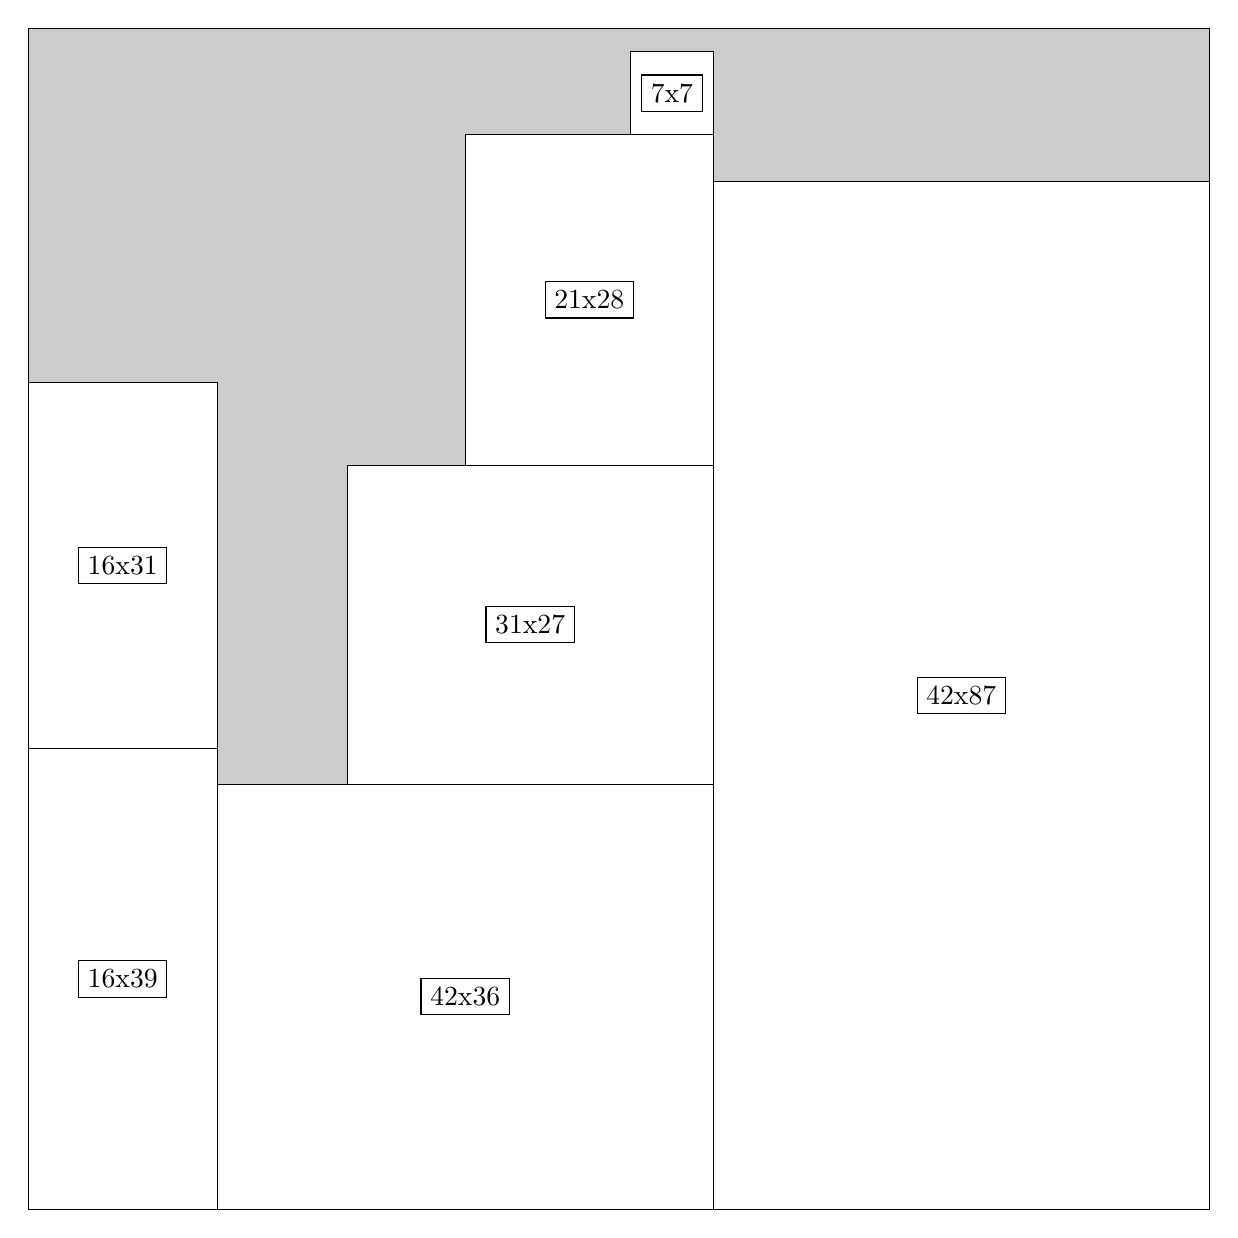
\begin{tikzpicture}[shorten >=1pt,scale=1.0,every node/.style={scale=1.0},->]
\tikzstyle{vertex}=[circle,fill=black!25,minimum size=14pt,inner sep=0pt]
\filldraw[fill=gray!40!white, draw=black] (0,0) rectangle (15.0,15.0);
\foreach \name/\x/\y/\w/\h in {42x87/8.7/0.0/6.3/13.049999999999999,42x36/2.4/0.0/6.3/5.3999999999999995,31x27/4.05/5.3999999999999995/4.6499999999999995/4.05,21x28/5.55/9.45/3.15/4.2,7x7/7.6499999999999995/13.65/1.05/1.05,16x39/0.0/0.0/2.4/5.85,16x31/0.0/5.85/2.4/4.6499999999999995}
\filldraw[fill=white!40!white, draw=black] (\x,\y) rectangle node[draw] (\name) {\name} ++(\w,\h);
\end{tikzpicture}


w =42 , h =87 , x =58 , y =0 , v =3654
\par
w =42 , h =36 , x =16 , y =0 , v =1512
\par
w =31 , h =27 , x =27 , y =36 , v =837
\par
w =21 , h =28 , x =37 , y =63 , v =588
\par
w =7 , h =7 , x =51 , y =91 , v =49
\par
w =16 , h =39 , x =0 , y =0 , v =624
\par
w =16 , h =31 , x =0 , y =39 , v =496
\par
\newpage


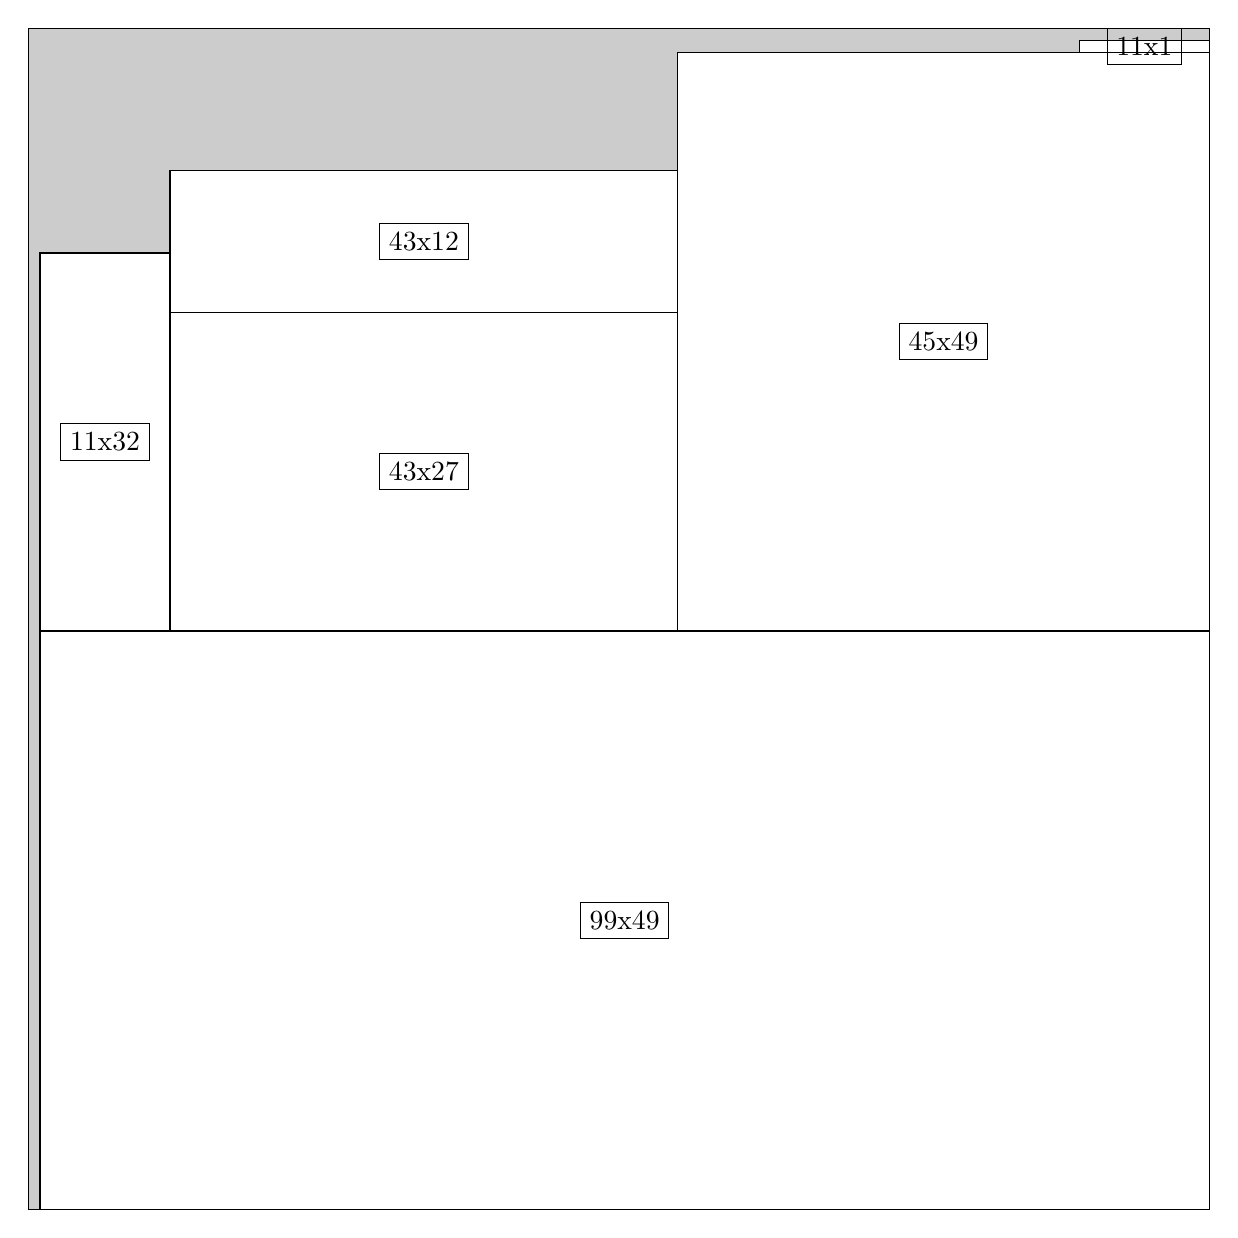
\begin{tikzpicture}[shorten >=1pt,scale=1.0,every node/.style={scale=1.0},->]
\tikzstyle{vertex}=[circle,fill=black!25,minimum size=14pt,inner sep=0pt]
\filldraw[fill=gray!40!white, draw=black] (0,0) rectangle (15.0,15.0);
\foreach \name/\x/\y/\w/\h in {99x49/0.15/0.0/14.85/7.35,45x49/8.25/7.35/6.75/7.35,11x1/13.35/14.7/1.65/0.15,43x27/1.7999999999999998/7.35/6.45/4.05,43x12/1.7999999999999998/11.4/6.45/1.7999999999999998,11x32/0.15/7.35/1.65/4.8}
\filldraw[fill=white!40!white, draw=black] (\x,\y) rectangle node[draw] (\name) {\name} ++(\w,\h);
\end{tikzpicture}


w =99 , h =49 , x =1 , y =0 , v =4851
\par
w =45 , h =49 , x =55 , y =49 , v =2205
\par
w =11 , h =1 , x =89 , y =98 , v =11
\par
w =43 , h =27 , x =12 , y =49 , v =1161
\par
w =43 , h =12 , x =12 , y =76 , v =516
\par
w =11 , h =32 , x =1 , y =49 , v =352
\par
\newpage


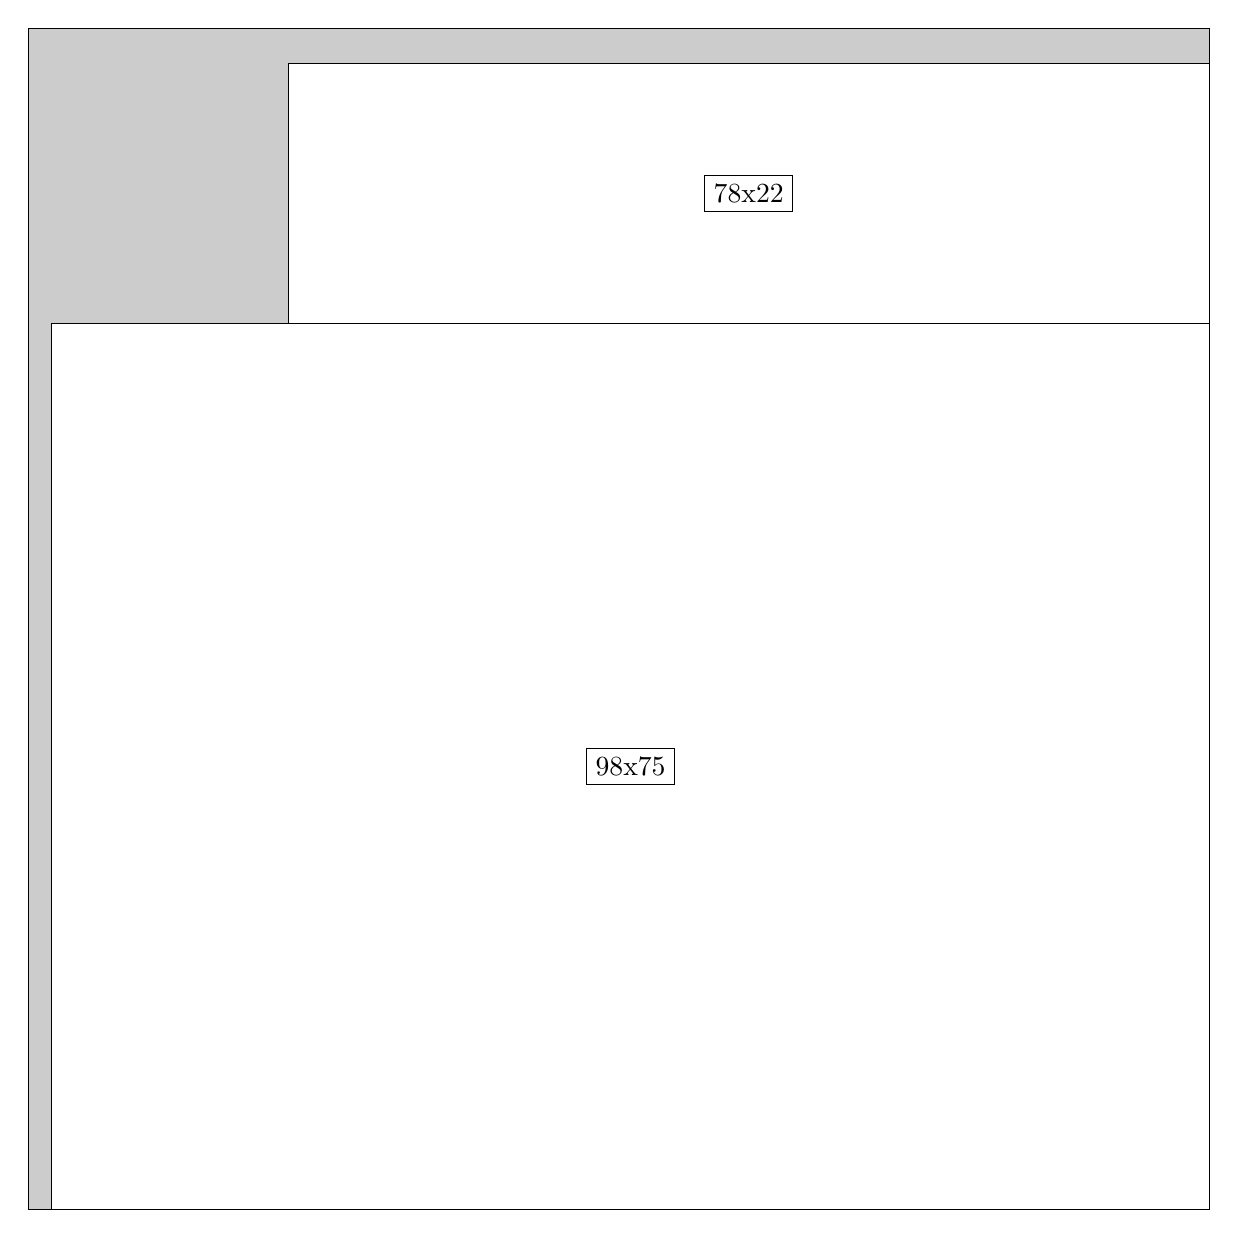
\begin{tikzpicture}[shorten >=1pt,scale=1.0,every node/.style={scale=1.0},->]
\tikzstyle{vertex}=[circle,fill=black!25,minimum size=14pt,inner sep=0pt]
\filldraw[fill=gray!40!white, draw=black] (0,0) rectangle (15.0,15.0);
\foreach \name/\x/\y/\w/\h in {98x75/0.3/0.0/14.7/11.25,78x22/3.3/11.25/11.7/3.3}
\filldraw[fill=white!40!white, draw=black] (\x,\y) rectangle node[draw] (\name) {\name} ++(\w,\h);
\end{tikzpicture}


w =98 , h =75 , x =2 , y =0 , v =7350
\par
w =78 , h =22 , x =22 , y =75 , v =1716
\par
\newpage


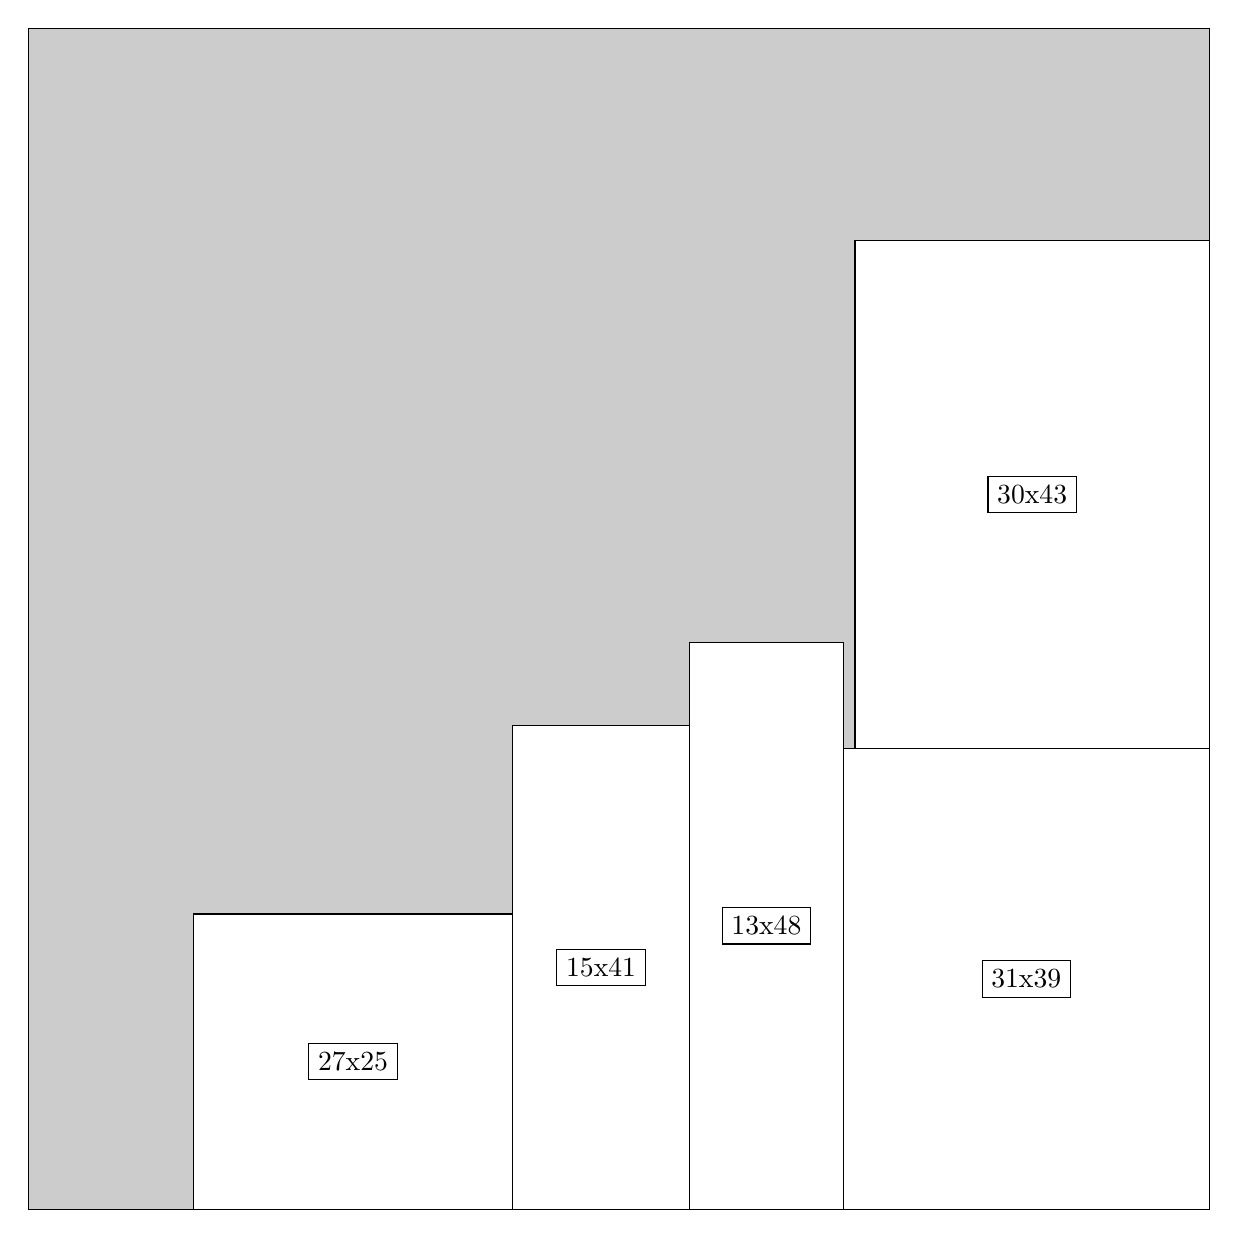
\begin{tikzpicture}[shorten >=1pt,scale=1.0,every node/.style={scale=1.0},->]
\tikzstyle{vertex}=[circle,fill=black!25,minimum size=14pt,inner sep=0pt]
\filldraw[fill=gray!40!white, draw=black] (0,0) rectangle (15.0,15.0);
\foreach \name/\x/\y/\w/\h in {31x39/10.35/0.0/4.6499999999999995/5.85,30x43/10.5/5.85/4.5/6.45,13x48/8.4/0.0/1.95/7.199999999999999,15x41/6.1499999999999995/0.0/2.25/6.1499999999999995,27x25/2.1/0.0/4.05/3.75}
\filldraw[fill=white!40!white, draw=black] (\x,\y) rectangle node[draw] (\name) {\name} ++(\w,\h);
\end{tikzpicture}


w =31 , h =39 , x =69 , y =0 , v =1209
\par
w =30 , h =43 , x =70 , y =39 , v =1290
\par
w =13 , h =48 , x =56 , y =0 , v =624
\par
w =15 , h =41 , x =41 , y =0 , v =615
\par
w =27 , h =25 , x =14 , y =0 , v =675
\par
\newpage


\end{document}